\documentclass[12pt]{amsart}
\usepackage{fullpage}
\usepackage{pbox}
\usepackage{graphicx}
\usepackage{booktabs} % Top and bottom rules for table
\usepackage{amsfonts, amsmath, amsthm, amssymb}
\usepackage{longtable,array,color,xcolor}
\usepackage[colorlinks = true,
            urlcolor  = blue]{hyperref}
\usepackage{verbatim}
\usepackage{enumerate}
\usepackage{lscape}
\newcommand\narrowstyle{\SetTracking{encoding=*}{-50}\lsstyle}

\setlength{\parindent}{0pt}

\begin{document}

\title{Math 320: Homework 5}
Due: October 21, 2016
\maketitle


Please read chapters 9 and 10 in the textbook 
and complete the following problems.

\begin{enumerate}

\item Problem 9.5

\begin{enumerate}
\item Solve graphically. We use the following code to plot
the image below:
\begin{verbatim}
x1 = 8:.1:13;
x2 = 0.5*x1 + 9.5;
x3 = .51*x1 + 9.4;
plot(x1,x2,x1,x3)
\end{verbatim}
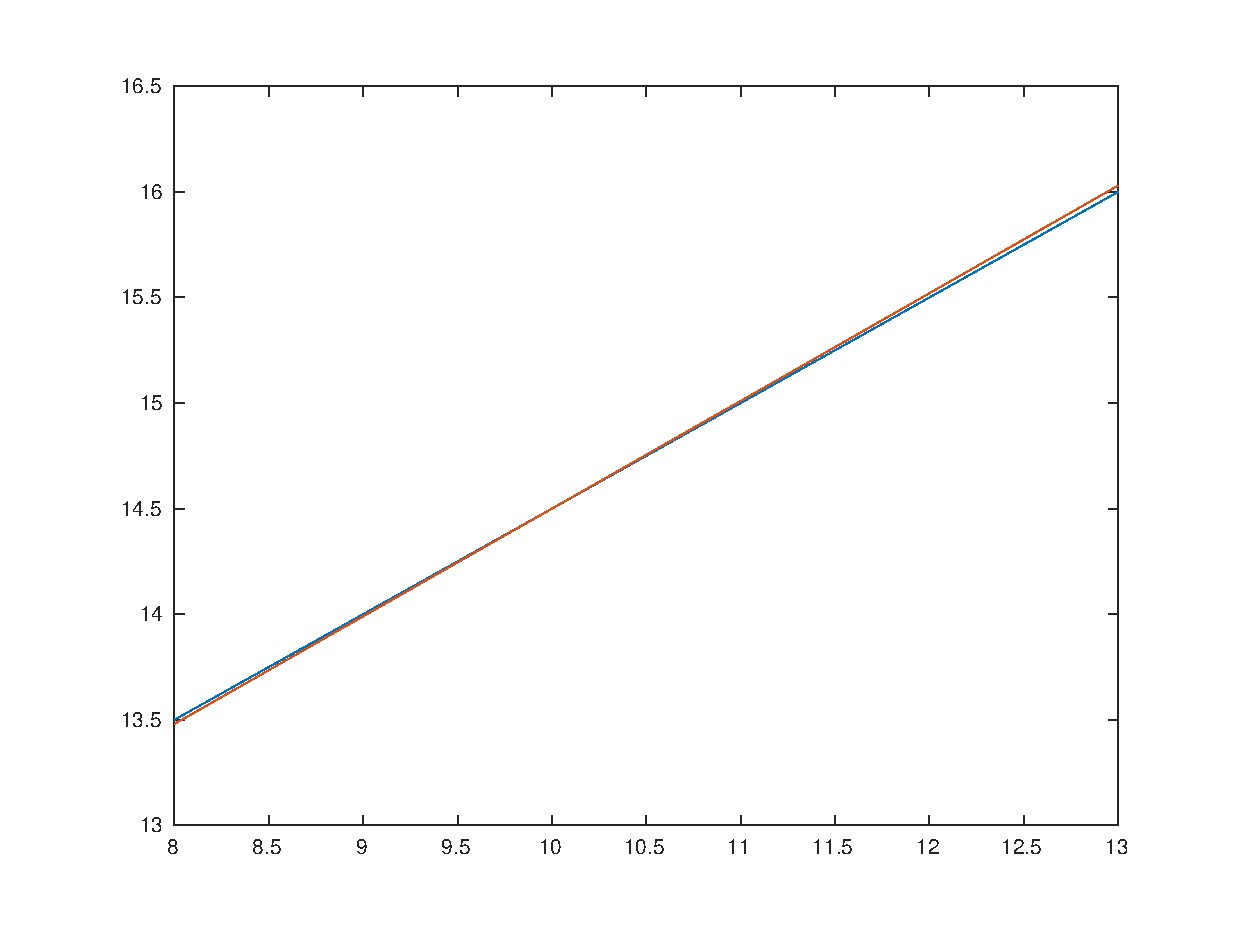
\includegraphics[width=.9\textwidth]{lines.eps}

From the picture, it seems that $x_1 = 10, x_2 = 14.5$ is the
solution.

\item Compute the determinant. The matrix form of the equation
is
\[ \left( \begin{array}{cc}
0.5 & -1 \\
1.02 & -2 \\
\end{array} \right)
\left( \begin{array}{c}
x_1 \\ x_2
\end{array}\right)
= \left( \begin{array}{c} -9.5 \\ -18.8 \end{array} \right).
\]

The determinant of the left-hand matrix is $0.02$.

\item On the basis of (a) and (b), I would guess that
the system is ill-conditioned; in particular, the condition
number is high. (Indeed, it is 314.5168, using 2-norm.)

\item Solve by the elimination of unknowns. Start by solving
$x_2 = 0.5 x_1  + 9.5$, then substitute into 
\[ 1.02x_1 -2(0.5 x_1 + 9.5) = -18.8 \iff 1.02x_1 - 1 x_1 - 19 = -18.8 \]
\[ \iff 0.02 x_1 = .2 \iff x_1 = 10 \Rightarrow x_2 = 14.5.\]

The solution is $(10,14.5)$ as guessed above.


\item Solve again, but with $a_{11}$ modified slightly to $0.52$.
This time: $x_2 = 0.52 x_1  + 9.5$

\[ 1.02x_1 -2(0.52 x_1 + 9.5) = -18.8 \iff 1.02x_1 - 1.04 x_1 - 19 = -18.8 \]
\[ \iff -0.02 x_1 = .2 \iff x_1 = -10 \Rightarrow x_2 = 4.3.\]

Because the system is so ill-conditioned, even a slight perturbation in
the coefficients can lead to a huge shift in the solution. Here, the
value of $a_{11}$ changed by $.02$ but the solution shifted by $20$ in the
$x_1$ coordinate, and $10.2$ in the $x_2$ coordinate. Poor condition makes
linear systems susceptible to being thrown way off by noise.

\end{enumerate}

\vfill
\pagebreak

\item Problem 10.12.
We have the LU factorization:
\[ A = LU = 
\left(\begin{array}{ccc}
1 & & \\
0.6667 & 1 & \\
-0.3333 & -0.3636 & 1 \\
\end{array}
\right) \left(\begin{array}{ccc}
3 & - 2 & 1 \\
& 7.3333 & -4.6667 \\
& & 3.6364 \\
\end{array}
\right) 
\]
\begin{enumerate}
\item The determinant of this product can be computed
as the product of the two determinants. Since both are
triangular, we need only multiply the diagonal elements
in the $U$ matrix. $3 \times 7.3333 \times 3.6364 = 80.0004$.

\item Solving $A x = b$ can be solved using $LUx = b \iff Ly = b$ and $Ux = y$. So we solve:
\[
\left(\begin{array}{ccc}
1 & & \\
0.6667 & 1 & \\
-0.3333 & -0.3636 & 1 \\
\end{array} \right) y = \left( \begin{array}{c}
-10 \\ 50 \\ -26
\end{array} \right) \]
Using forward-subsitution, we find $y_1 = -10$, then
$-6.667 + y_2 = 50 \Rightarrow y_2 = 56.667$, then
$3.333 -20.6041 + y_3 = -26 \Rightarrow y_3 = -8.7289$.

Then, we use back-substitution to solve the following system:
\[
\right) \left(\begin{array}{ccc}
3 & - 2 & 1 \\
& 7.3333 & -4.6667 \\
& & 3.6364 \\
\end{array}
\right)x  =
\left( \begin{array}{c}
-10 \\ 56.667 \\ -8.7289
\end{array} \right)
\]
First, we have $x_3 = -2.4004$, then $7.3333 x_2 - 4.6667
\times(-2.4004) = 56.667 \Rightarrow x_2 = 6.200$, and then
$3\times x_1 + (-2)\times (6.2000) + 1 \times (-2.4004) = 
-10 \Rightarrow x_1 = 1.600$. \\

The solution therefore is $(1.600, 6.200,-2.400)$.

\end{enumerate}

\vfill
\pagebreak

\item Problem 10.13

\[A = U^T U = \left( \begin{array}{ccc}
2 & -1 & 0 \\ -1 & 2 & -1 \\ 0 & -1 & 2 
\end{array} \right)\]

We can use MATLAB command {\tt chol(A)} to find
the following Cholesky factorization:
\[U = \left( \begin{array}{ccc}
1.4142 & -0.7071 & 0 \\ 0 & 1.2247 & -0.8165 \\ 0 & 0 & 1.1547
\end{array} \right)\]

To find this explicitly, we solve the system of equations:
 \begin{align*}
u_{11}^2 & =  a_{11} & \Rightarrow & u_{11}  =  \sqrt{2} \\
u_{11}u_{12} & =  a_{12}  & \Rightarrow & \sqrt{2} u_{12} =  -1 & \Rightarrow &  u_{12} = \frac{-1}{\sqrt{2}} \\
u_{11}u_{13} & =  a_{13}  & \Rightarrow & \sqrt{2} u_{13} =  0 & \Rightarrow & u_{13} = 0 \\
u_{12}^2 + u_{22}^2 & =  a_{22}  & \Rightarrow & \frac{1}{2} +  u_{22}^2 =  2 & \Rightarrow& u_{22} = \sqrt{\frac{3}{2}} \\
u_{12} u_{13} + u_{22} u_{23} & =  a_{23} & \Rightarrow & 0 + \sqrt{\frac{3}{2}} u_{23}  = -1 & \Rightarrow & u_{23} = - \sqrt{\frac{2}{3}} \\
u_{13}^2 + u_{23}^2 + u_{33}^2 & =  a_{33} & \Rightarrow & 0 + \frac{2}{3} + u_{33}^2 = 2 & \Rightarrow & u_{33} = \frac{2}{\sqrt{3}}\\
\end{align*}


\vfill
\pagebreak 


\item Take three points in the plane with distinct x-coordinates 
so that they are not collinear. The statement "these three 
points define a parabola" is equivalent to a certain matrix 
equation involving a 3 x 3 matrix.

\begin{enumerate}
\item What is the matrix equation?

Let the three points be $(x_1,y_1),(x_2,y_2)$, and $(x_3,y_3)$.
Then assuming they lie on a parabola $y = ax^2 + bx + c$ means 
the following matrix equation holds:

\[ \left( \begin{array}{ccc}
x_1^2 & x_1 & 1 \\
x_2^2 & x_2 & 1 \\
x_3^2 & x_3 & 1 \\
\end{array}\right) \left( \begin{array}{c}
a \\ b \\ c \end{array} \right)
= \left( \begin{array}{c} y_1 & y_2 & y_3
\end{array} \right) \]

\item  Using this equation, write a MATLAB 
function {\tt parab} which takes as input 
three points and gives output a string 
{\tt "y=ax\^{}2 + bx + c"} where a,b, and c 
are replaced by numbers so that all three points 
lie on the corresponding parabola.


The MATLAB code used to produce this output is
below:

\begin{verbatim}
function s = parab(x1,y1,x2,y2,x3,y3)
%takes three points in the plane as input
%outputs a string defining the parabola

M = [x1^2 x1 1; x2^2 x2 1; x3^2 x3 1];
V = [y1, y2, y3];
x = (M\V')';
s = sprintf('y = %f x^2 + %f x + %f',...
x(1),x(2),x(3));
\end{verbatim}

\item Evaluate your function given the three 
points $(0,1),(2,-3)$, and $(3,2)$.

The output for this evaluation is 

{\begin{verbatim} y = 2.333333 x^2 + -6.666667 x + 1.000000\end{verbatim}

\end{enumerate}


\end{enumerate}
\end{document}
